\documentclass[]{book}
\usepackage{lmodern}
\usepackage{amssymb,amsmath}
\usepackage{ifxetex,ifluatex}
\usepackage{fixltx2e} % provides \textsubscript
\ifnum 0\ifxetex 1\fi\ifluatex 1\fi=0 % if pdftex
  \usepackage[T1]{fontenc}
  \usepackage[utf8]{inputenc}
\else % if luatex or xelatex
  \ifxetex
    \usepackage{mathspec}
  \else
    \usepackage{fontspec}
  \fi
  \defaultfontfeatures{Ligatures=TeX,Scale=MatchLowercase}
\fi
% use upquote if available, for straight quotes in verbatim environments
\IfFileExists{upquote.sty}{\usepackage{upquote}}{}
% use microtype if available
\IfFileExists{microtype.sty}{%
\usepackage{microtype}
\UseMicrotypeSet[protrusion]{basicmath} % disable protrusion for tt fonts
}{}
\usepackage[margin=1in]{geometry}
\usepackage{hyperref}
\hypersetup{unicode=true,
            pdftitle={Recommendations from Floodnet Project 1-6},
            pdfauthor={Martin Durocher},
            pdfborder={0 0 0},
            breaklinks=true}
\urlstyle{same}  % don't use monospace font for urls
\usepackage{natbib}
\bibliographystyle{apalike}
\usepackage{color}
\usepackage{fancyvrb}
\newcommand{\VerbBar}{|}
\newcommand{\VERB}{\Verb[commandchars=\\\{\}]}
\DefineVerbatimEnvironment{Highlighting}{Verbatim}{commandchars=\\\{\}}
% Add ',fontsize=\small' for more characters per line
\usepackage{framed}
\definecolor{shadecolor}{RGB}{248,248,248}
\newenvironment{Shaded}{\begin{snugshade}}{\end{snugshade}}
\newcommand{\AlertTok}[1]{\textcolor[rgb]{0.94,0.16,0.16}{#1}}
\newcommand{\AnnotationTok}[1]{\textcolor[rgb]{0.56,0.35,0.01}{\textbf{\textit{#1}}}}
\newcommand{\AttributeTok}[1]{\textcolor[rgb]{0.77,0.63,0.00}{#1}}
\newcommand{\BaseNTok}[1]{\textcolor[rgb]{0.00,0.00,0.81}{#1}}
\newcommand{\BuiltInTok}[1]{#1}
\newcommand{\CharTok}[1]{\textcolor[rgb]{0.31,0.60,0.02}{#1}}
\newcommand{\CommentTok}[1]{\textcolor[rgb]{0.56,0.35,0.01}{\textit{#1}}}
\newcommand{\CommentVarTok}[1]{\textcolor[rgb]{0.56,0.35,0.01}{\textbf{\textit{#1}}}}
\newcommand{\ConstantTok}[1]{\textcolor[rgb]{0.00,0.00,0.00}{#1}}
\newcommand{\ControlFlowTok}[1]{\textcolor[rgb]{0.13,0.29,0.53}{\textbf{#1}}}
\newcommand{\DataTypeTok}[1]{\textcolor[rgb]{0.13,0.29,0.53}{#1}}
\newcommand{\DecValTok}[1]{\textcolor[rgb]{0.00,0.00,0.81}{#1}}
\newcommand{\DocumentationTok}[1]{\textcolor[rgb]{0.56,0.35,0.01}{\textbf{\textit{#1}}}}
\newcommand{\ErrorTok}[1]{\textcolor[rgb]{0.64,0.00,0.00}{\textbf{#1}}}
\newcommand{\ExtensionTok}[1]{#1}
\newcommand{\FloatTok}[1]{\textcolor[rgb]{0.00,0.00,0.81}{#1}}
\newcommand{\FunctionTok}[1]{\textcolor[rgb]{0.00,0.00,0.00}{#1}}
\newcommand{\ImportTok}[1]{#1}
\newcommand{\InformationTok}[1]{\textcolor[rgb]{0.56,0.35,0.01}{\textbf{\textit{#1}}}}
\newcommand{\KeywordTok}[1]{\textcolor[rgb]{0.13,0.29,0.53}{\textbf{#1}}}
\newcommand{\NormalTok}[1]{#1}
\newcommand{\OperatorTok}[1]{\textcolor[rgb]{0.81,0.36,0.00}{\textbf{#1}}}
\newcommand{\OtherTok}[1]{\textcolor[rgb]{0.56,0.35,0.01}{#1}}
\newcommand{\PreprocessorTok}[1]{\textcolor[rgb]{0.56,0.35,0.01}{\textit{#1}}}
\newcommand{\RegionMarkerTok}[1]{#1}
\newcommand{\SpecialCharTok}[1]{\textcolor[rgb]{0.00,0.00,0.00}{#1}}
\newcommand{\SpecialStringTok}[1]{\textcolor[rgb]{0.31,0.60,0.02}{#1}}
\newcommand{\StringTok}[1]{\textcolor[rgb]{0.31,0.60,0.02}{#1}}
\newcommand{\VariableTok}[1]{\textcolor[rgb]{0.00,0.00,0.00}{#1}}
\newcommand{\VerbatimStringTok}[1]{\textcolor[rgb]{0.31,0.60,0.02}{#1}}
\newcommand{\WarningTok}[1]{\textcolor[rgb]{0.56,0.35,0.01}{\textbf{\textit{#1}}}}
\usepackage{longtable,booktabs}
\usepackage{graphicx,grffile}
\makeatletter
\def\maxwidth{\ifdim\Gin@nat@width>\linewidth\linewidth\else\Gin@nat@width\fi}
\def\maxheight{\ifdim\Gin@nat@height>\textheight\textheight\else\Gin@nat@height\fi}
\makeatother
% Scale images if necessary, so that they will not overflow the page
% margins by default, and it is still possible to overwrite the defaults
% using explicit options in \includegraphics[width, height, ...]{}
\setkeys{Gin}{width=\maxwidth,height=\maxheight,keepaspectratio}
\IfFileExists{parskip.sty}{%
\usepackage{parskip}
}{% else
\setlength{\parindent}{0pt}
\setlength{\parskip}{6pt plus 2pt minus 1pt}
}
\setlength{\emergencystretch}{3em}  % prevent overfull lines
\providecommand{\tightlist}{%
  \setlength{\itemsep}{0pt}\setlength{\parskip}{0pt}}
\setcounter{secnumdepth}{5}
% Redefines (sub)paragraphs to behave more like sections
\ifx\paragraph\undefined\else
\let\oldparagraph\paragraph
\renewcommand{\paragraph}[1]{\oldparagraph{#1}\mbox{}}
\fi
\ifx\subparagraph\undefined\else
\let\oldsubparagraph\subparagraph
\renewcommand{\subparagraph}[1]{\oldsubparagraph{#1}\mbox{}}
\fi

%%% Use protect on footnotes to avoid problems with footnotes in titles
\let\rmarkdownfootnote\footnote%
\def\footnote{\protect\rmarkdownfootnote}

%%% Change title format to be more compact
\usepackage{titling}

% Create subtitle command for use in maketitle
\newcommand{\subtitle}[1]{
  \posttitle{
    \begin{center}\large#1\end{center}
    }
}

\setlength{\droptitle}{-2em}

  \title{Recommendations from Floodnet Project 1-6}
    \pretitle{\vspace{\droptitle}\centering\huge}
  \posttitle{\par}
    \author{Martin Durocher}
    \preauthor{\centering\large\emph}
  \postauthor{\par}
      \predate{\centering\large\emph}
  \postdate{\par}
    \date{2019-01-28}

\usepackage{booktabs}

\usepackage{amsthm}
\newtheorem{theorem}{Theorem}[chapter]
\newtheorem{lemma}{Lemma}[chapter]
\theoremstyle{definition}
\newtheorem{definition}{Definition}[chapter]
\newtheorem{corollary}{Corollary}[chapter]
\newtheorem{proposition}{Proposition}[chapter]
\theoremstyle{definition}
\newtheorem{example}{Example}[chapter]
\theoremstyle{definition}
\newtheorem{exercise}{Exercise}[chapter]
\theoremstyle{remark}
\newtheorem*{remark}{Remark}
\newtheorem*{solution}{Solution}
\begin{document}
\maketitle

{
\setcounter{tocdepth}{1}
\tableofcontents
}
\hypertarget{welcome}{%
\chapter{Welcome}\label{welcome}}

\textbf{IN CONSTRUCTION}

A description of the objectives of the Floodnet Project can be found at
the \href{http://www.nsercfloodnet.ca/}{Floodnet webpage}

PDF and EPUB versions of this book can be downloaded from the
\href{https://github.com/floodnetProject16/recommendations/tree/master/docs}{GitHub
repository}

\hypertarget{amax}{%
\chapter{Annual maximums}\label{amax}}

\hypertarget{introduction}{%
\section{Introduction}\label{introduction}}

In this document I will show how to use \texttt{floodnetRfa} to perform
at-site frequency analysis using annual maximum discharge. First we will
extract the annual maximums from the daily discharge data of the
Saint-John River at Fort Kent (NB). Note that incomplet year with
missing observations will be removed. In total 88 annual maximums are
extracted and showed in a histogram.

\begin{Shaded}
\begin{Highlighting}[]
\KeywordTok{library}\NormalTok{(floodnetRfa)}

\NormalTok{anData <-}\StringTok{ }\KeywordTok{ExtractAmax}\NormalTok{(flow }\OperatorTok{~}\StringTok{ }\NormalTok{date, flowStJohn, }\DataTypeTok{tol =} \DecValTok{365}\NormalTok{)}

\NormalTok{npDens <-}\StringTok{ }\KeywordTok{density}\NormalTok{(anData}\OperatorTok{$}\NormalTok{flow)}

\KeywordTok{hist}\NormalTok{(anData}\OperatorTok{$}\NormalTok{flow, }
     \DataTypeTok{freq =} \OtherTok{FALSE}\NormalTok{, }
     \DataTypeTok{main =} \StringTok{''}\NormalTok{, }
     \DataTypeTok{xlab =} \StringTok{'Discharge'}\NormalTok{,}
     \DataTypeTok{ylim =} \KeywordTok{c}\NormalTok{(}\DecValTok{0}\NormalTok{, }\KeywordTok{max}\NormalTok{(npDens}\OperatorTok{$}\NormalTok{y)))}

\KeywordTok{lines}\NormalTok{(npDens, }\DataTypeTok{col =} \DecValTok{2}\NormalTok{, }\DataTypeTok{lwd =} \DecValTok{2}\NormalTok{)}
\end{Highlighting}
\end{Shaded}

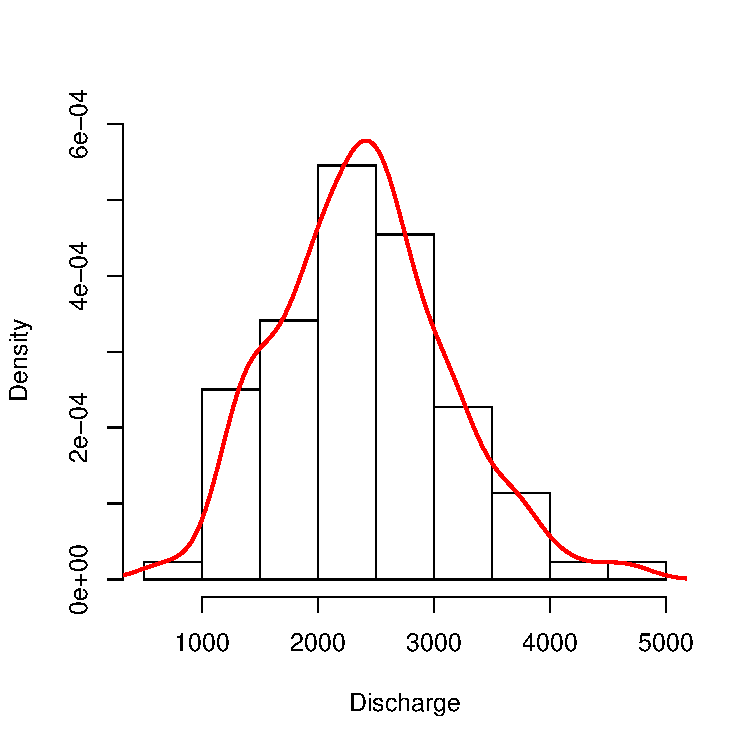
\includegraphics{FloodnetProject16_files/figure-latex/unnamed-chunk-1-1.pdf}

In stationary situation, the annual maximums are assumed to be
independant and identically distributed. Risk is then measure in terms
of return period that characterizes the average time separating two
events of the same magnitude. In practice this is equivalent to
calculate the probability \(p = 1-1/T\) of a fitted distribution. The
test of Mann-Kendall is frequently performed to verify if the data
contains a significant trend that would invalidate the assumption of
stationarity. The present data have a p-value of 0.21, which does not
suggest the present of a trend.

\begin{Shaded}
\begin{Highlighting}[]
\KeywordTok{plot}\NormalTok{(flow}\OperatorTok{~}\NormalTok{date, anData)}
\end{Highlighting}
\end{Shaded}

\begin{figure}
\centering
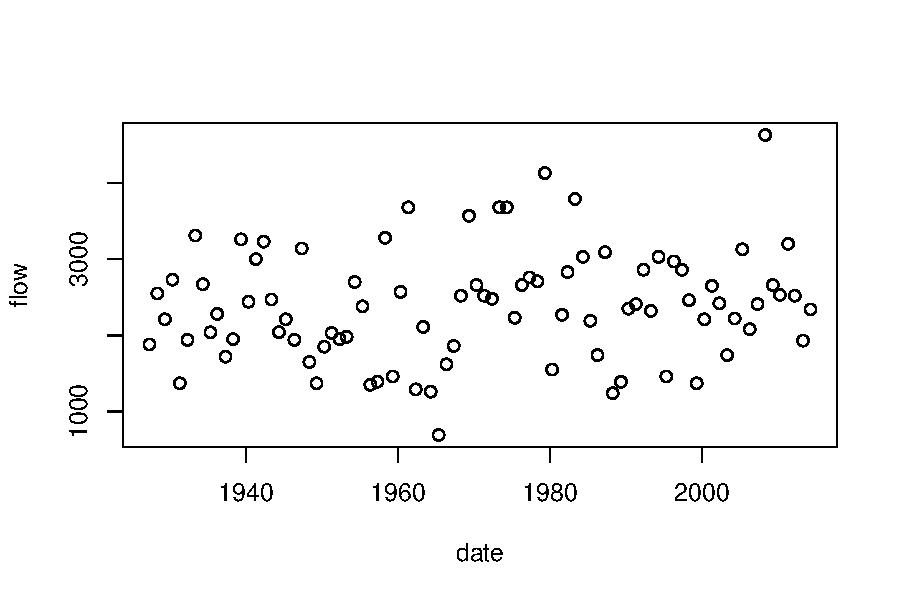
\includegraphics{FloodnetProject16_files/figure-latex/amax-mkendall-1.pdf}
\caption{\label{fig:amax-mkendall}Trend in the annual maximums}
\end{figure}

\begin{Shaded}
\begin{Highlighting}[]
\KeywordTok{MKendall}\NormalTok{(anData}\OperatorTok{$}\NormalTok{flow)}
\end{Highlighting}
\end{Shaded}

\begin{verbatim}
## 
## 
## Mann-Kendall Test for trend
## S:  346
## p-value:  0.2136
\end{verbatim}

\hypertarget{estimation-of-the-flood-quantiles}{%
\section{Estimation of the flood
quantiles}\label{estimation-of-the-flood-quantiles}}

According to extreme value theory, as the number of annual maximums
increase, their distribution converge to Generalized Extreme Value (GEV)
distribution

\begin{equation}
F(x) = \exp\left\{ - \left[ 1 - \kappa \left(\frac{x-\xi}{\alpha} \right) \right]^{1/\kappa} \right\}
\label{eq:amax-gevcdf}
\end{equation}

The GEV distribution in Equation \eqref{eq:amax-gevcdf} can be fitted
using the \texttt{FitAmax} function. The example below shows how the
parameter are estimated using the maximum likelihood method. See for
instance \citep{coles_introduction_2001}. A brief summary of the fitted
model is reported, including the estimated parameter, their standard
deviation and the sample L-moments.

\begin{Shaded}
\begin{Highlighting}[]
\NormalTok{fit <-}\StringTok{ }\KeywordTok{FitAmax}\NormalTok{(anData}\OperatorTok{$}\NormalTok{flow, }\StringTok{'gev'}\NormalTok{, }\DataTypeTok{method =} \StringTok{'mle'}\NormalTok{)}

\KeywordTok{print}\NormalTok{(fit)}
\end{Highlighting}
\end{Shaded}

\begin{verbatim}
## 
## At-site frequency analysis
## 
## Distribution: gev 
## AIC: 1411 
## Method: mle
## Estimate:
##        xi     alpha     kappa 
## 2101.3761  668.9518    0.1667 
## 
## Std.err:
##       xi    alpha    kappa 
## 78.39437 54.31311  0.06214 
## 
## Lmoments:
##     l1  lcv     lsk    lkt
## 1 2390 0.17 0.05924 0.1399
\end{verbatim}

The flood quantile of the GEV distribution can be obtained from the
formula

\[
x_T = \mu + \frac{\alpha}{\xi}\left[ 1+\log(1/T)^\kappa \right] .
\] These predicted value are computed using the \texttt{predict}
function. In the example below show the flood quantile for return period
2, 5, 10, 20, 50 and 100. The standard deviation of the flood quantiles
is estimated using the Delta method that assume that the estimated
parameter follow a Normal distribution.

\begin{Shaded}
\begin{Highlighting}[]
\NormalTok{yhat <-}\StringTok{ }\KeywordTok{predict}\NormalTok{(fit, }\DataTypeTok{se =} \OtherTok{TRUE}\NormalTok{, }\DataTypeTok{ci =} \StringTok{'delta'}\NormalTok{)}
\end{Highlighting}
\end{Shaded}

\begin{table}

\caption{\label{tab:amax-yhat}Predicted return levels}
\centering
\begin{tabular}[t]{r|r|r|r}
\hline
pred & se & lower & upper\\
\hline
2339.216 & 82.44124 & 2177.634 & 2500.798\\
\hline
2989.156 & 99.81724 & 2793.518 & 3184.794\\
\hline
3356.637 & 117.79148 & 3125.770 & 3587.504\\
\hline
3668.464 & 144.52611 & 3385.198 & 3951.730\\
\hline
4020.327 & 193.47341 & 3641.126 & 4399.528\\
\hline
4250.404 & 238.46296 & 3783.025 & 4717.783\\
\hline
\end{tabular}
\end{table}

\hypertarget{verification-of-the-model}{%
\section{Verification of the model}\label{verification-of-the-model}}

The return level plot in \ref{fig:amax-gevreturnlevel} provide a visual
assessment of the fitted distribution by comparing the sample and the
predicted flood quantiles. The graphic below shows a good agreement
between the two.

\begin{Shaded}
\begin{Highlighting}[]
\KeywordTok{plot}\NormalTok{(fit, }\DataTypeTok{ci =} \OtherTok{TRUE}\NormalTok{)}
\end{Highlighting}
\end{Shaded}

\begin{figure}
\centering
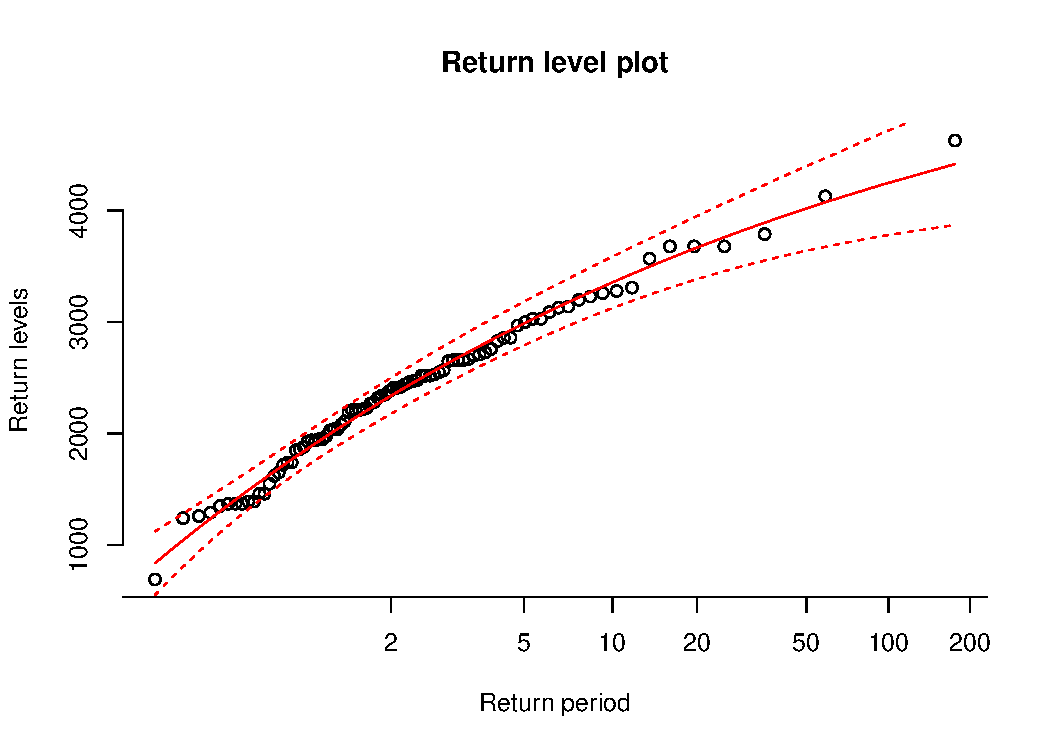
\includegraphics{FloodnetProject16_files/figure-latex/amax-gevreturnlevel-1.pdf}
\caption{\label{fig:amax-gevreturnlevel}Return level plot for Saint-John
River at Fort Kent, NB.}
\end{figure}

Another diagnostic to ensure that the GEV distribution is appropriate is
the Anderson-Darling test. The p-value superior to 0.05 indicates that
the hypothesis of a GEV cannot be rejected.

\begin{Shaded}
\begin{Highlighting}[]
\NormalTok{## Time consuming when estimated by 'mle'}
\KeywordTok{GofTest}\NormalTok{(fit, }\DataTypeTok{nsim =} \DecValTok{500}\NormalTok{)}
\end{Highlighting}
\end{Shaded}

\begin{verbatim}
## 
## Goodness-of-fit test for annual maxima
##  
## Test = Anderson-Darling 
## Distribution = gev
## statistic : 0.266 
## p-value : 0.602
\end{verbatim}

\bibliography{book.bib}


\end{document}
